设计文档
\chapter{项目概述}

随着电子商务的快速发展,各种电商平台层出不穷,同一个商品在不同的平台上价格差异很大,用户往往需要在多个平台上比价才能找到最优惠的商品。本项目旨在为用户提供一个商品比价的工具,用户可以通过输入商品名称,获取该商品在不同电商平台上的价格信息,从而帮助用户快速找到最优惠的商品。

本项目名为 “寻惠” (DisFinder),旨在帮助用户找到最优惠的商品。

\chapter{项目总体需求}

\begin{enumerate}
  \item 用户输入商品名称,系统返回该商品在不同电商平台上的价格信息。
  \item 能够显示历史价格信息,帮助用户了解商品价格走势。
  \item 用户可以关注商品,系统会定时推送商品价格变动信息。
  \item 支持用户注册、登录、修改密码等功能。
  \item 支持移动网页端访问。
\end{enumerate}

\chapter{设计细节}

\section{模块设计}

总体分为前端和后端两个部分,前端负责用户交互,后端负责数据处理。其中后端还包括数据采集模块和数据库模块。

\subsection{前端模块}

前端主要包括以下几个页面。

\begin{enumerate}
  \item 登录页面:用户登录、注册功能。
  \item 商品搜索页面:用户输入商品名称,返回一系列满足要求的商品缩略信息,供用户选择对应的商品。
  \item 商品详情页面:展示该商品的详细信息、各平台价格信息、历史价格走势等,并可以选择将商品添加到心愿单。
  \item 用户中心页面:展示用户信息,提供修改密码、退出登录、管理电商平台账户等功能
  \item 心愿单界面:展示用户关注的商品信息,提供取消关注、查看商品详情等功能。
\end{enumerate}

\subsection{后端模块}

后端主要包括以下几个模块。

\begin{enumerate}
  \item 鉴权模块:负责校验用户登录状态,保护用户数据安全。
  \item API 响应模块:负责处理前端请求,返回相应的数据。
  \item 数据采集模块:负责从各电商平台上采集商品价格信息。
  \item 数据操作模块:负责对数据库进行增删改查操作。
  \item 数据库模块:负责存储用户信息、商品信息、价格信息等。
  \item 定时任务模块:负责定时更新商品价格信息,推送商品价格变动信息。
\end{enumerate}

\subsection{技术栈}

\begin{itemize}
  \item 前端:Next.js
  \item 后端:go
  \item 数据库:MySQL,使用 GORM 进行操作。
  \item 数据采集:Python
\end{itemize}

\section{数据模型设计}

\subsection{模型设计细节}

主要涉及到以下数据模型:

\subsubsection{User: 用户信息}

\begin{itemize}
  \item UID
  \item Name
  \item email
  \item Password
\end{itemize}

\subsubsection{Product: 商品信息}

\begin{itemize}
  \item PID
  \item Name
  \item Description
\end{itemize}

\subsubsection{Platform: 电商平台信息}

\begin{itemize}
  \item ID
  \item Name
\end{itemize}

\subsubsection{PriceHistory: 商品价格历史信息}

\begin{itemize}
  \item PID
  \item PlatformID
  \item Date
  \item Price
\end{itemize}

\subsubsection{WishList: 用户关注的商品信息}

\begin{itemize}
  \item UID
  \item PID
\end{itemize}

\subsubsection{UserPlatform: 用户绑定的电商平台账户信息}

\begin{itemize}
  \item UID
  \item PlatformID
  \item Account
  \item Password
\end{itemize}

\subsection{GORM 设计}

由于我使用 GORM 进行数据库操作,因此只需要在 GO 中定义好数据模型,GORM 会自动创建对应的表。

\begin{codebox}{}{cool}
\begin{amzcode}{go}
type User struct {
    ID        uint           `json:"id" gorm:"column:id;primary_key;AUTO_INCREMENT"`
    Name      string         `json:"name" gorm:"column:name;type:varchar(255);not null"`
    Password  string         `json:"password" gorm:"column:password;type:varchar(255);not null"`
    Email     string         `json:"email" gorm:"column:email;type:varchar(255);unique;not null"`
    Wishlist  []Product      `json:"wishlist" gorm:"manytomany:wishlists;"`
    Platforms []UserPlatform `json:"platform" gorm:"foreignKey:UserID"`
}
\end{amzcode}
\end{codebox}

\begin{codebox}{}{cool}
\begin{amzcode}{go}
type Product struct {
    ID          uint   `json:"id" gorm:"column:id;primary_key;AUTO_INCREMENT"`
    Name        string `json:"name" gorm:"column:name;type:varchar(255);not null"`
    Description string `json:"description" gorm:"column:description;type:varchar(1023);not null"`
    Picture     string `json:"picture" gorm:"column:picture;type:varchar(255);not null"`
    Users       []User `json:"users" gorm:"many2many:wishlists;"`
}

\end{amzcode}
\end{codebox}

\begin{codebox}{}{cool}
\begin{amzcode}{go}
type Platform struct {
    ID   uint   `json:"id" gorm:"column:id;primary_key;AUTO_INCREMENT"`
    Name string `json:"name" gorm:"column:name;type:varchar(255);not null"`
}
\end{amzcode}
\end{codebox}

\begin{codebox}{}{cool}
\begin{amzcode}{go}
type PriceHistory struct {
    ProductID  uint      `json:"product_id" gorm:"column:product_id;type:int;not null;primary_key"`
    PlatformID uint      `json:"platform_id" gorm:"column:platform_id;type:int;not null;primary_key"`
    Date       null.Time `json:"date" gorm:"column:date;type:date;not null"`
    Price      float64   `json:"price" gorm:"column:price;type:decimal(10,2);not null"`
}
\end{amzcode}
\end{codebox}

\begin{codebox}{}{cool}
\begin{amzcode}{go}
type UserPlatform struct {
    UserID     uint   `json:"user_id" gorm:"column:user_id;type:int;not null"`
    PlatformID uint   `json:"platform_id" gorm:"column:platform_id;type:int;not null"`
    Account    string `json:"account" gorm:"column:account;type:varchar(255);not null"`
    Password   string `json:"password" gorm:"column:password;type:varchar(255);not null"`
}
\end{amzcode}
\end{codebox}

其中 Wishlist 的表由 GORM 自动创建,不需要额外定义。

\section{接口设计}

我使用 Apifox 工具进行接口设计,对数据模型和接口进行统一管理。

[Apifox 接口文档](https://apifox.com/apidoc/project-5427055/)

\begin{figure}[H]
\centering
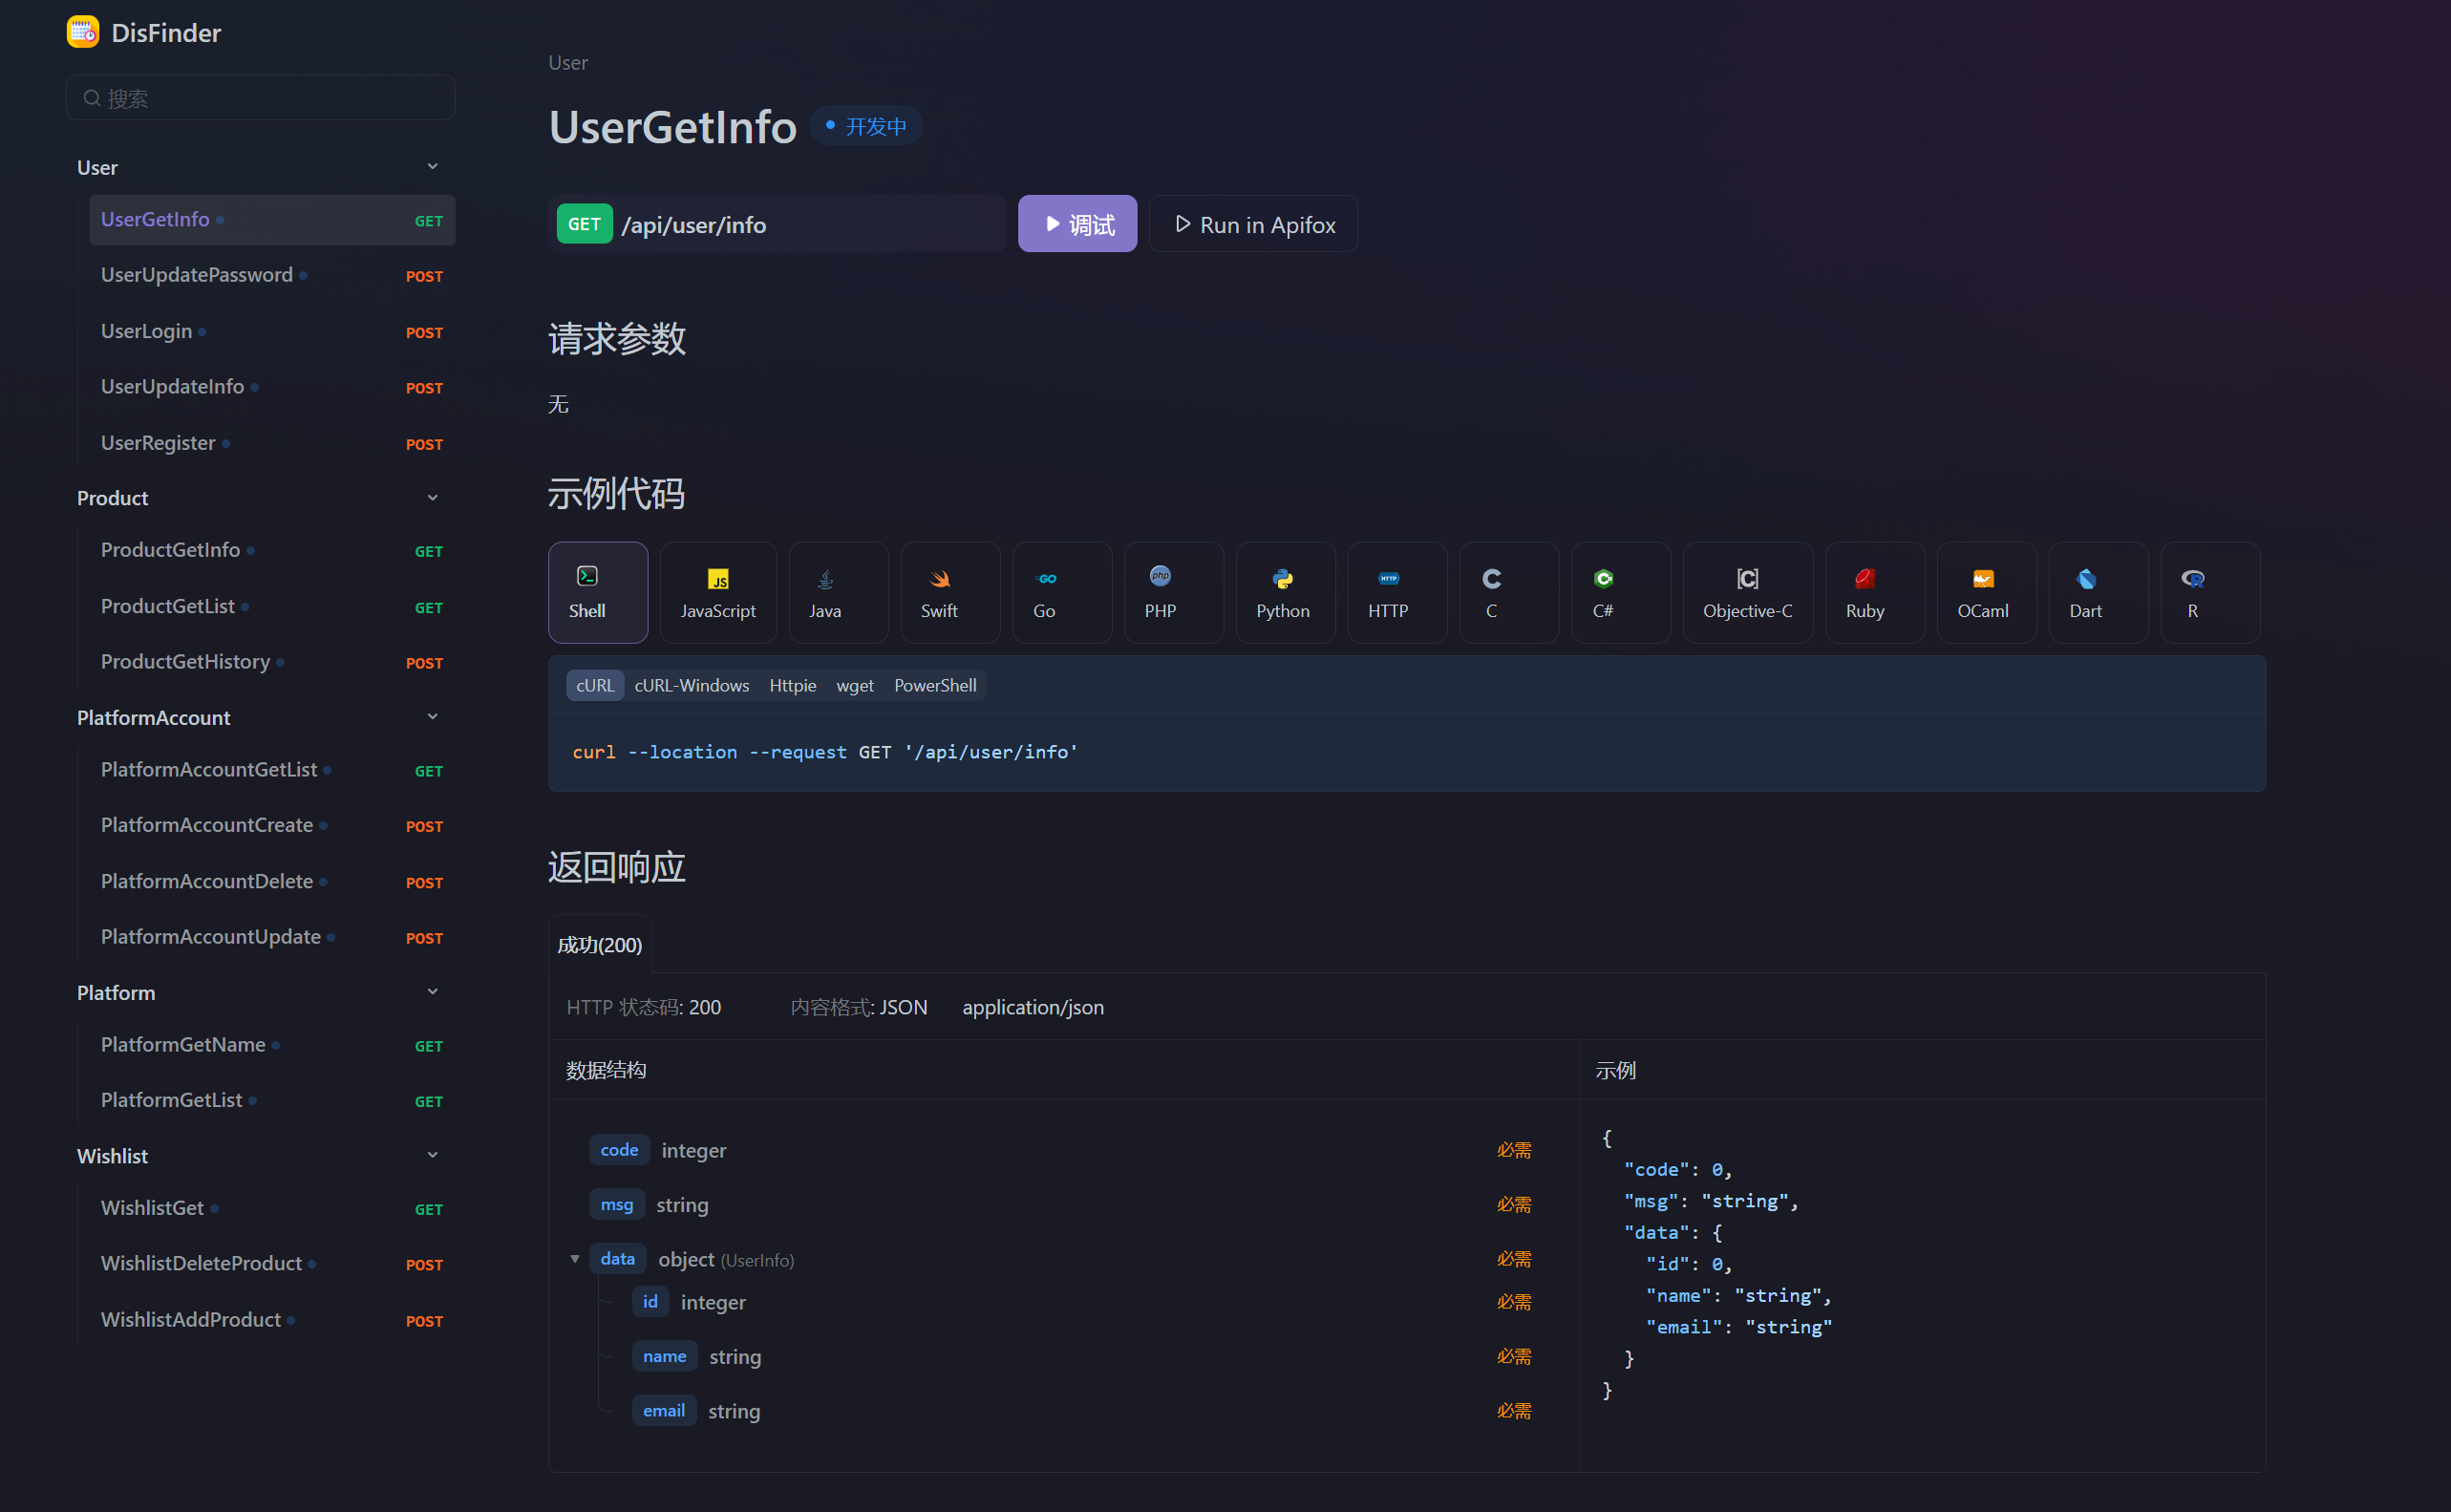
\includegraphics[width=0.5\textwidth]{assets/design/apifox.png}
\caption{Apifox 接口文档展示}
\end{figure}

\subsubsection{用户信息接口}

\begin{itemize}
  \item 用户注册
  \item 用户登录
  \item 修改密码
  \item 用户信息查询
  \item 用户信息修改
  \item 登出
\end{itemize}

\subsubsection{电商平台账户接口}

\begin{itemize}
  \item 查询电商平台账户信息
  \item 绑定电商平台账户
  \item 解绑电商平台账户
  \item 修改电商平台账户信息
\end{itemize}

\subsubsection{电商平台接口}

\begin{itemize}
  \item 获取所有电商平台
\end{itemize}

\subsubsection{心愿单接口}

\begin{itemize}
  \item 查询心愿单
  \item 从心愿单中删除商品
  \item 添加商品到心愿单
\end{itemize}

\subsubsection{商品接口}

\begin{itemize}
  \item 查询商品信息
  \item 查询商品历史价格信息
  \item 批量获取商品
\end{itemize}

\section{前端设计}

前端主要使用 Next.js 进行开发,使用 NextUI 进行 UI 设计。

主要包含以下几个页面:

\begin{itemize}
  \item 主页面
  \item 用户登录页面
  \item 用户信息页面
  \item 商品搜索页面
  \item 商品详情页面
  \item 心愿单页面
\end{itemize}

以下是页面设计草案,不代表最终效果。

\subsubsection{主页面}

\begin{figure}[H]
\centering
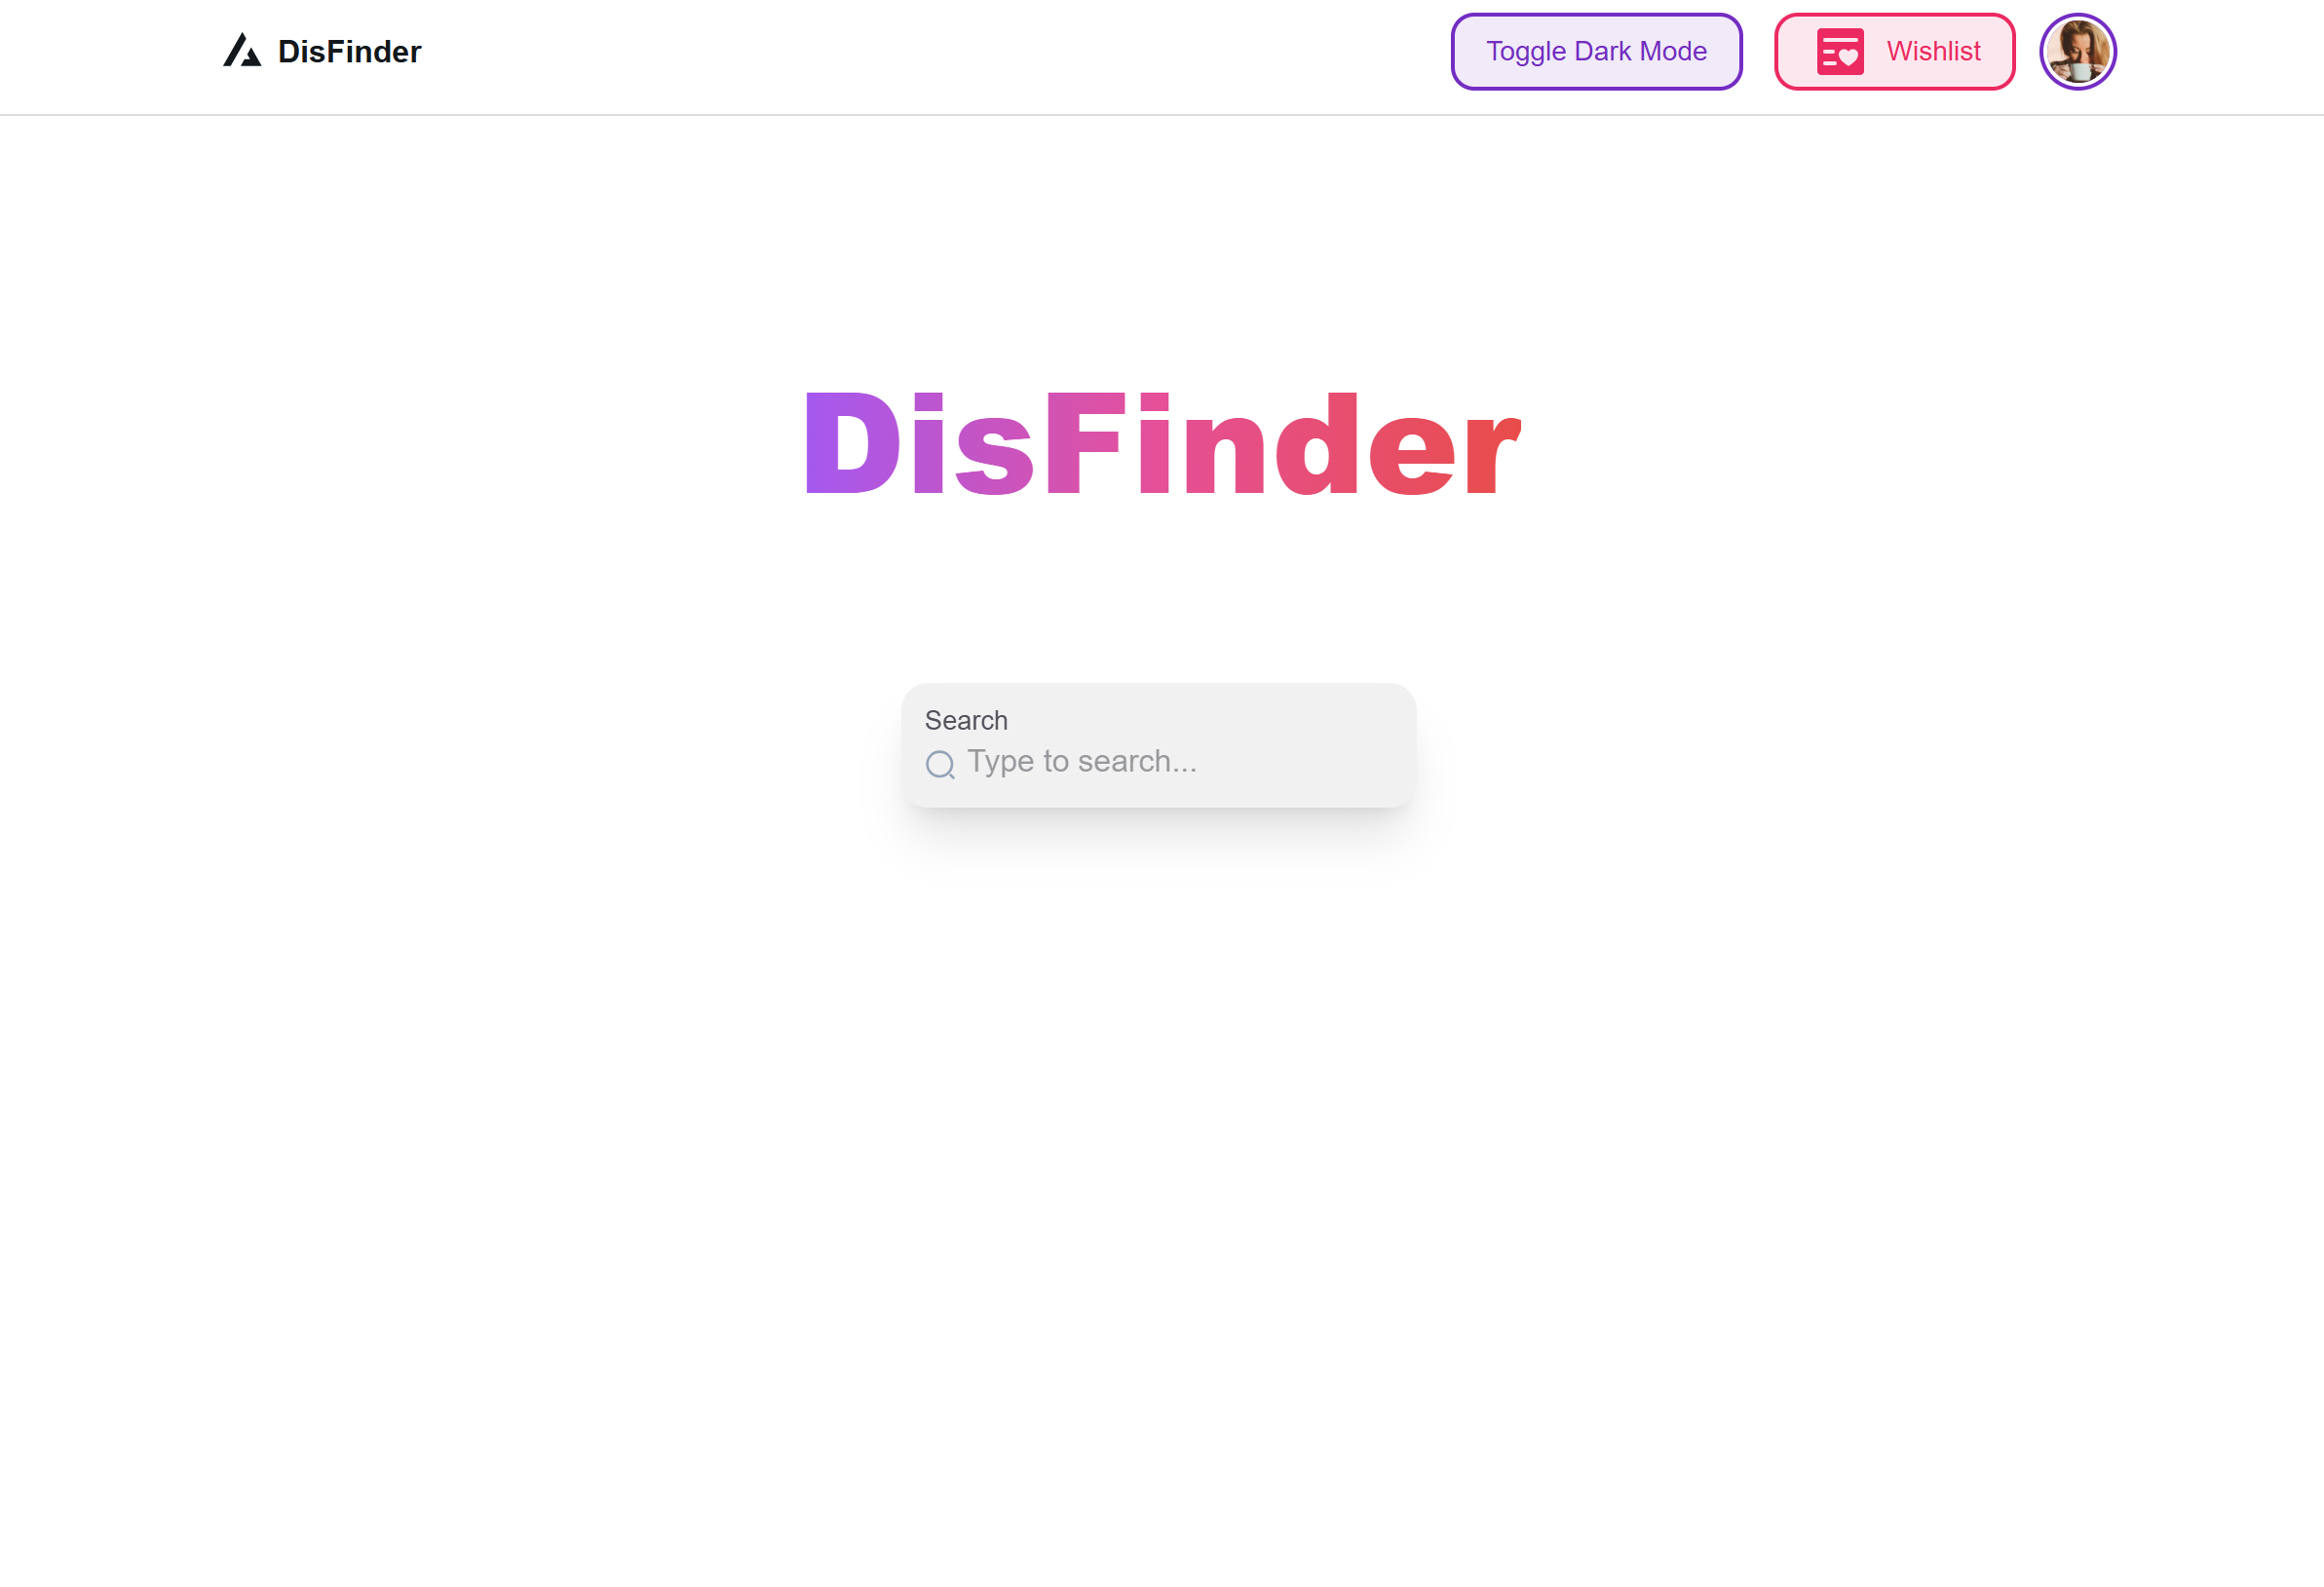
\includegraphics[width=0.5\textwidth]{assets/design/homepage.png}
\caption{主界面示例}
\end{figure}

\subsubsection{用户登录/注册界面}

\begin{figure}[H]
\centering
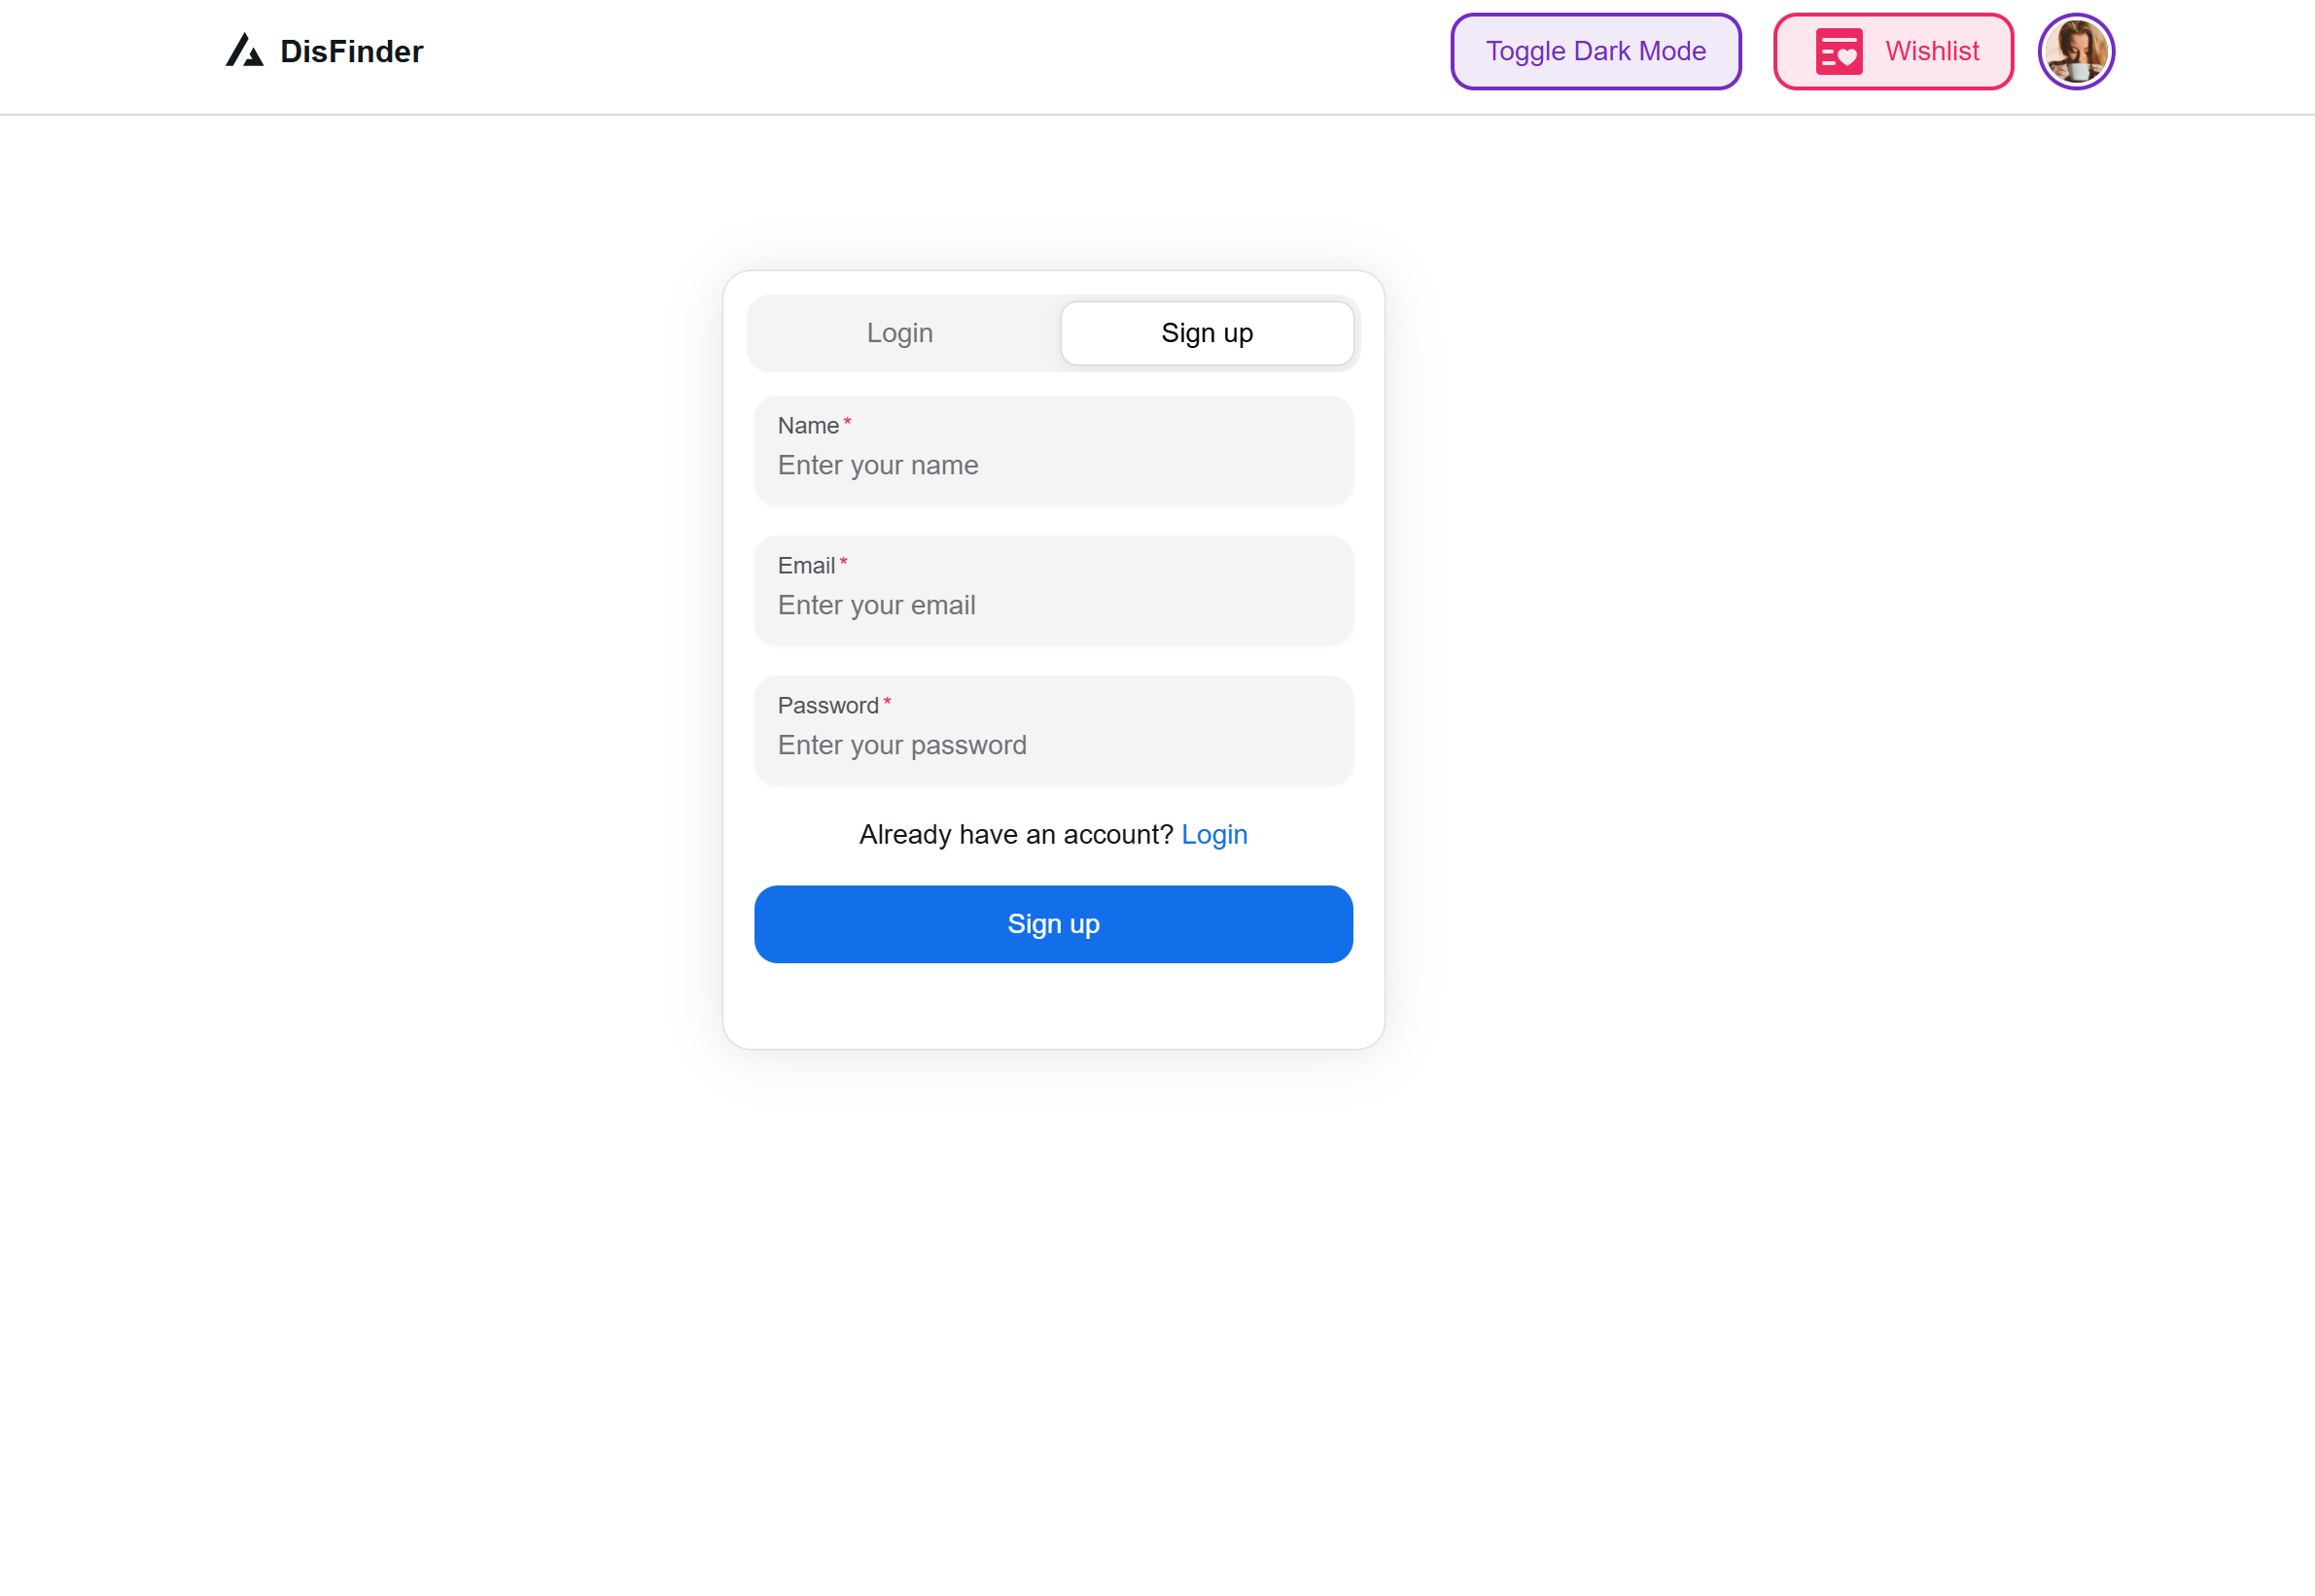
\includegraphics[width=0.5\textwidth]{assets/design/authpage.png}
\caption{用户登录/注册界面示例}
\end{figure}

\subsubsection{用户信息界面}

\begin{figure}[H]
\centering
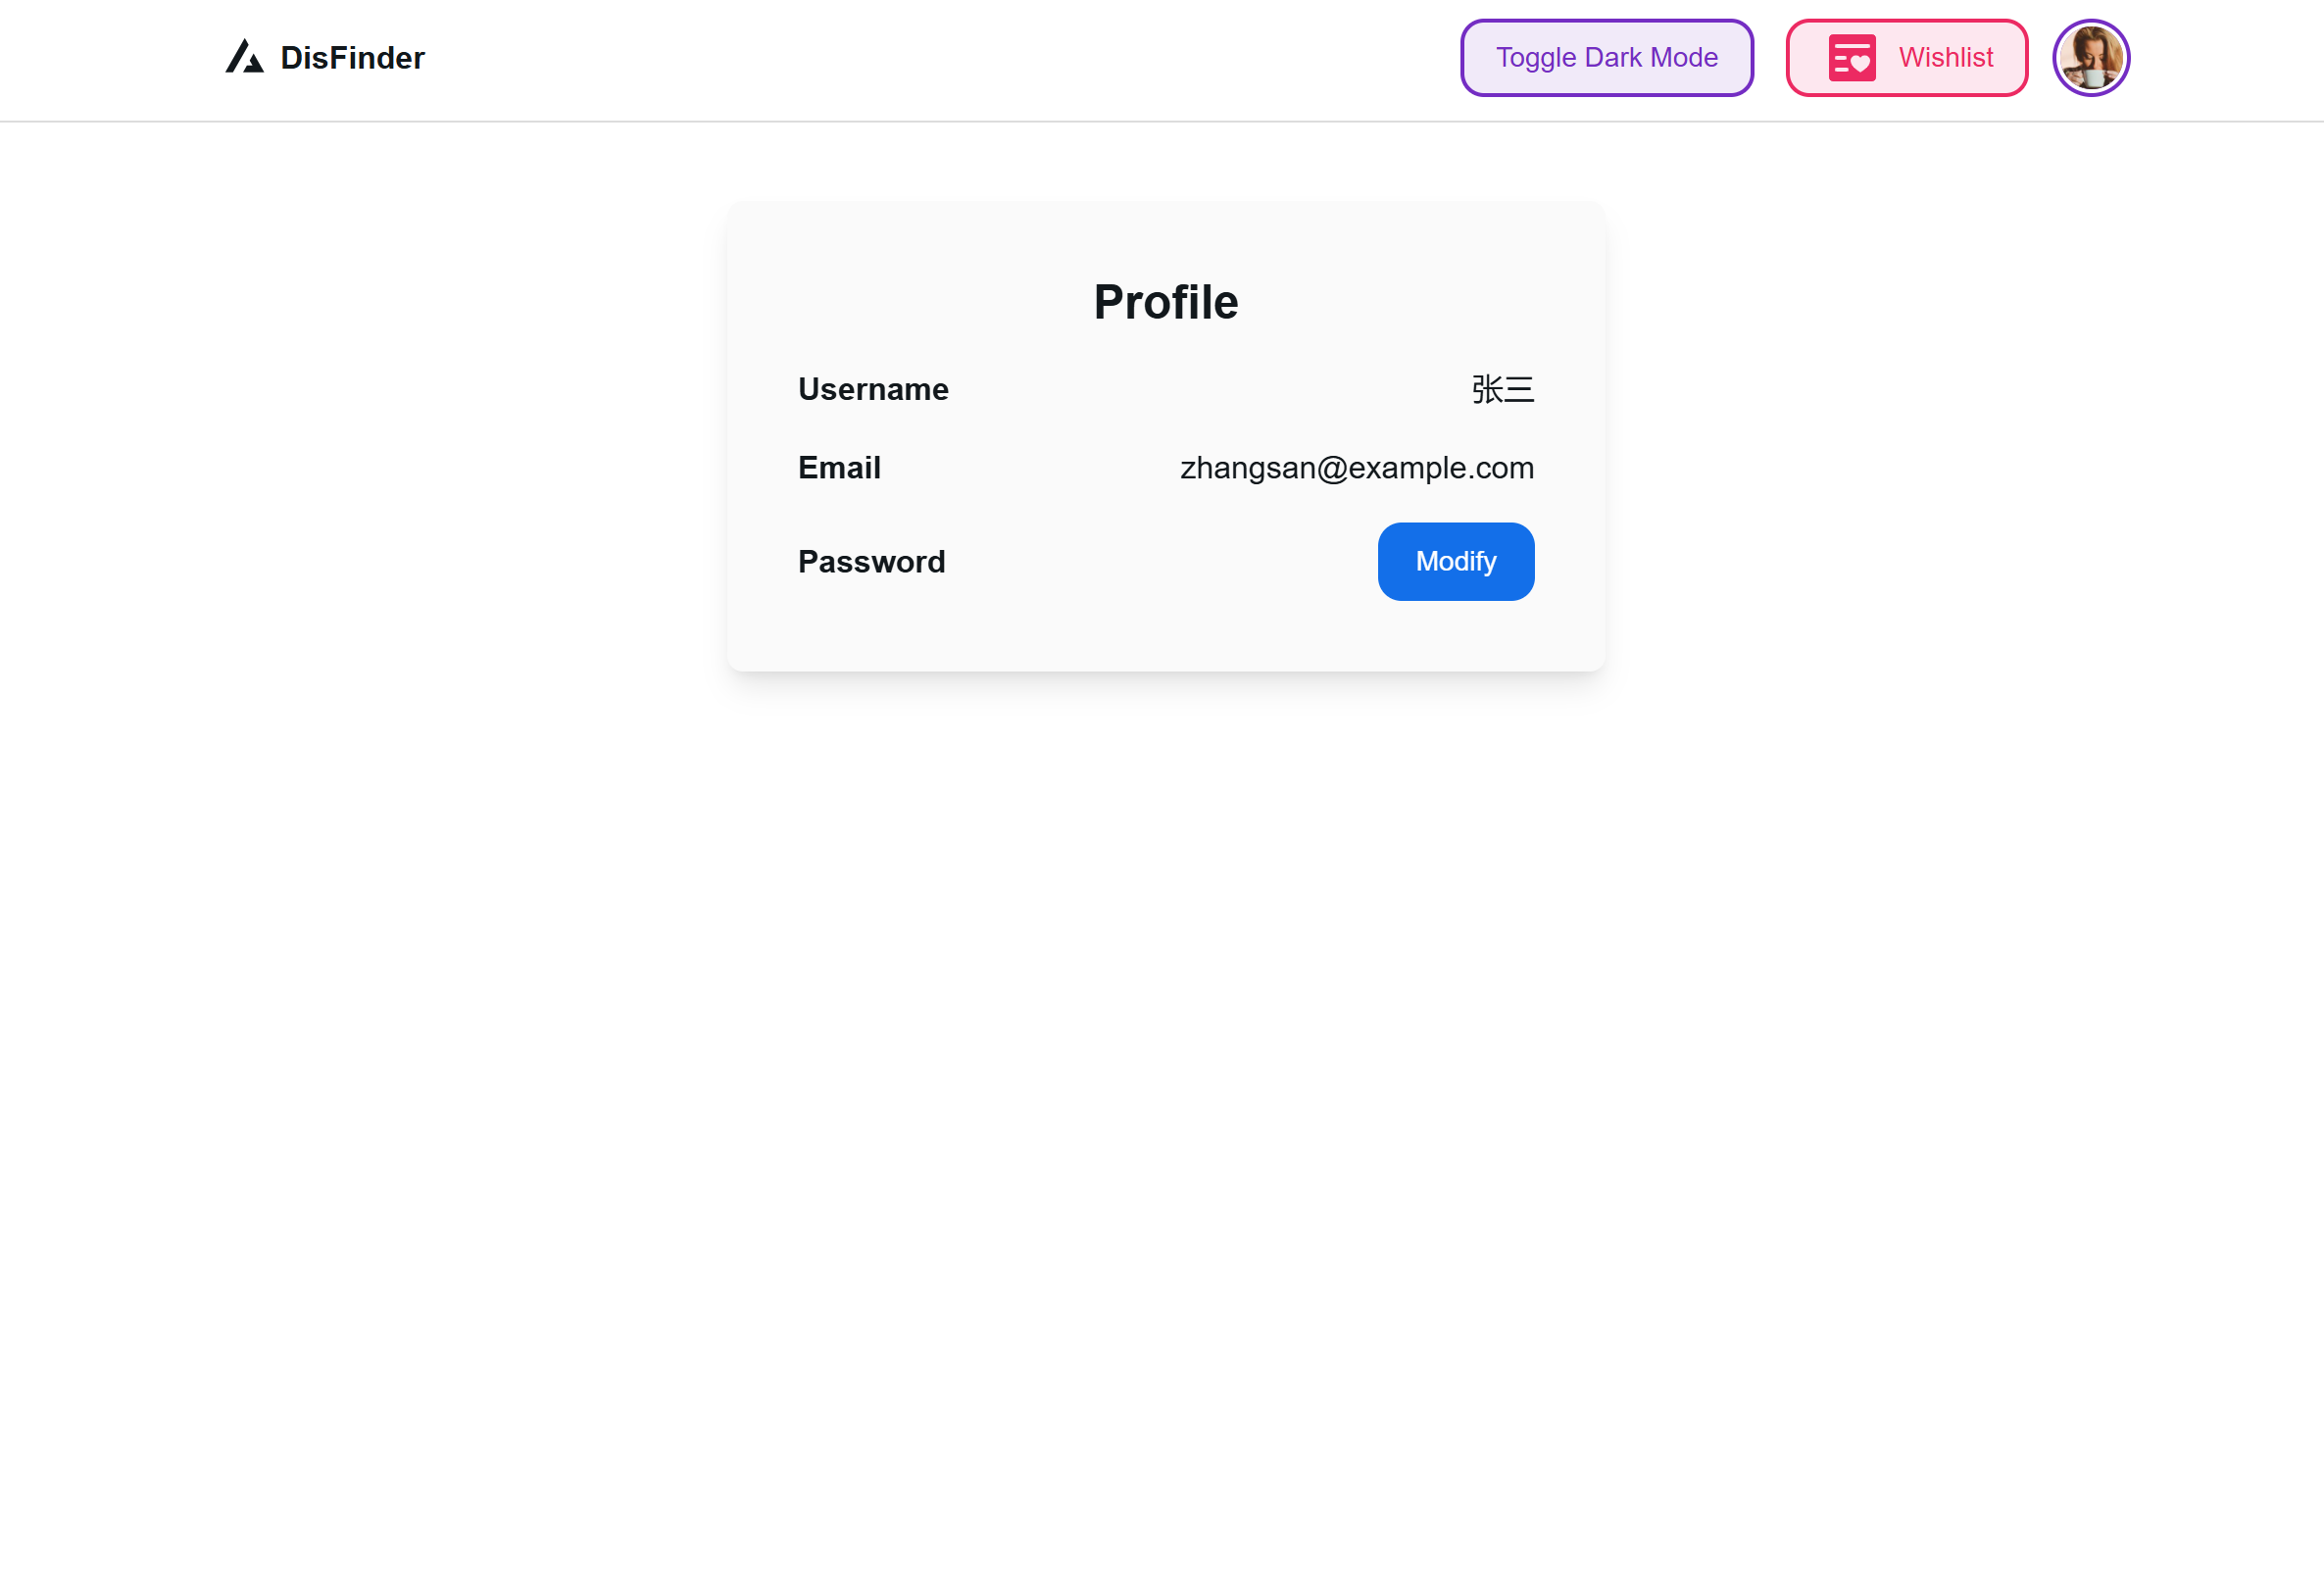
\includegraphics[width=0.5\textwidth]{assets/design/userpage.png}
\caption{用户信息界面示例}
\end{figure}

\subsubsection{商品搜索界面}

\begin{figure}[H]
\centering
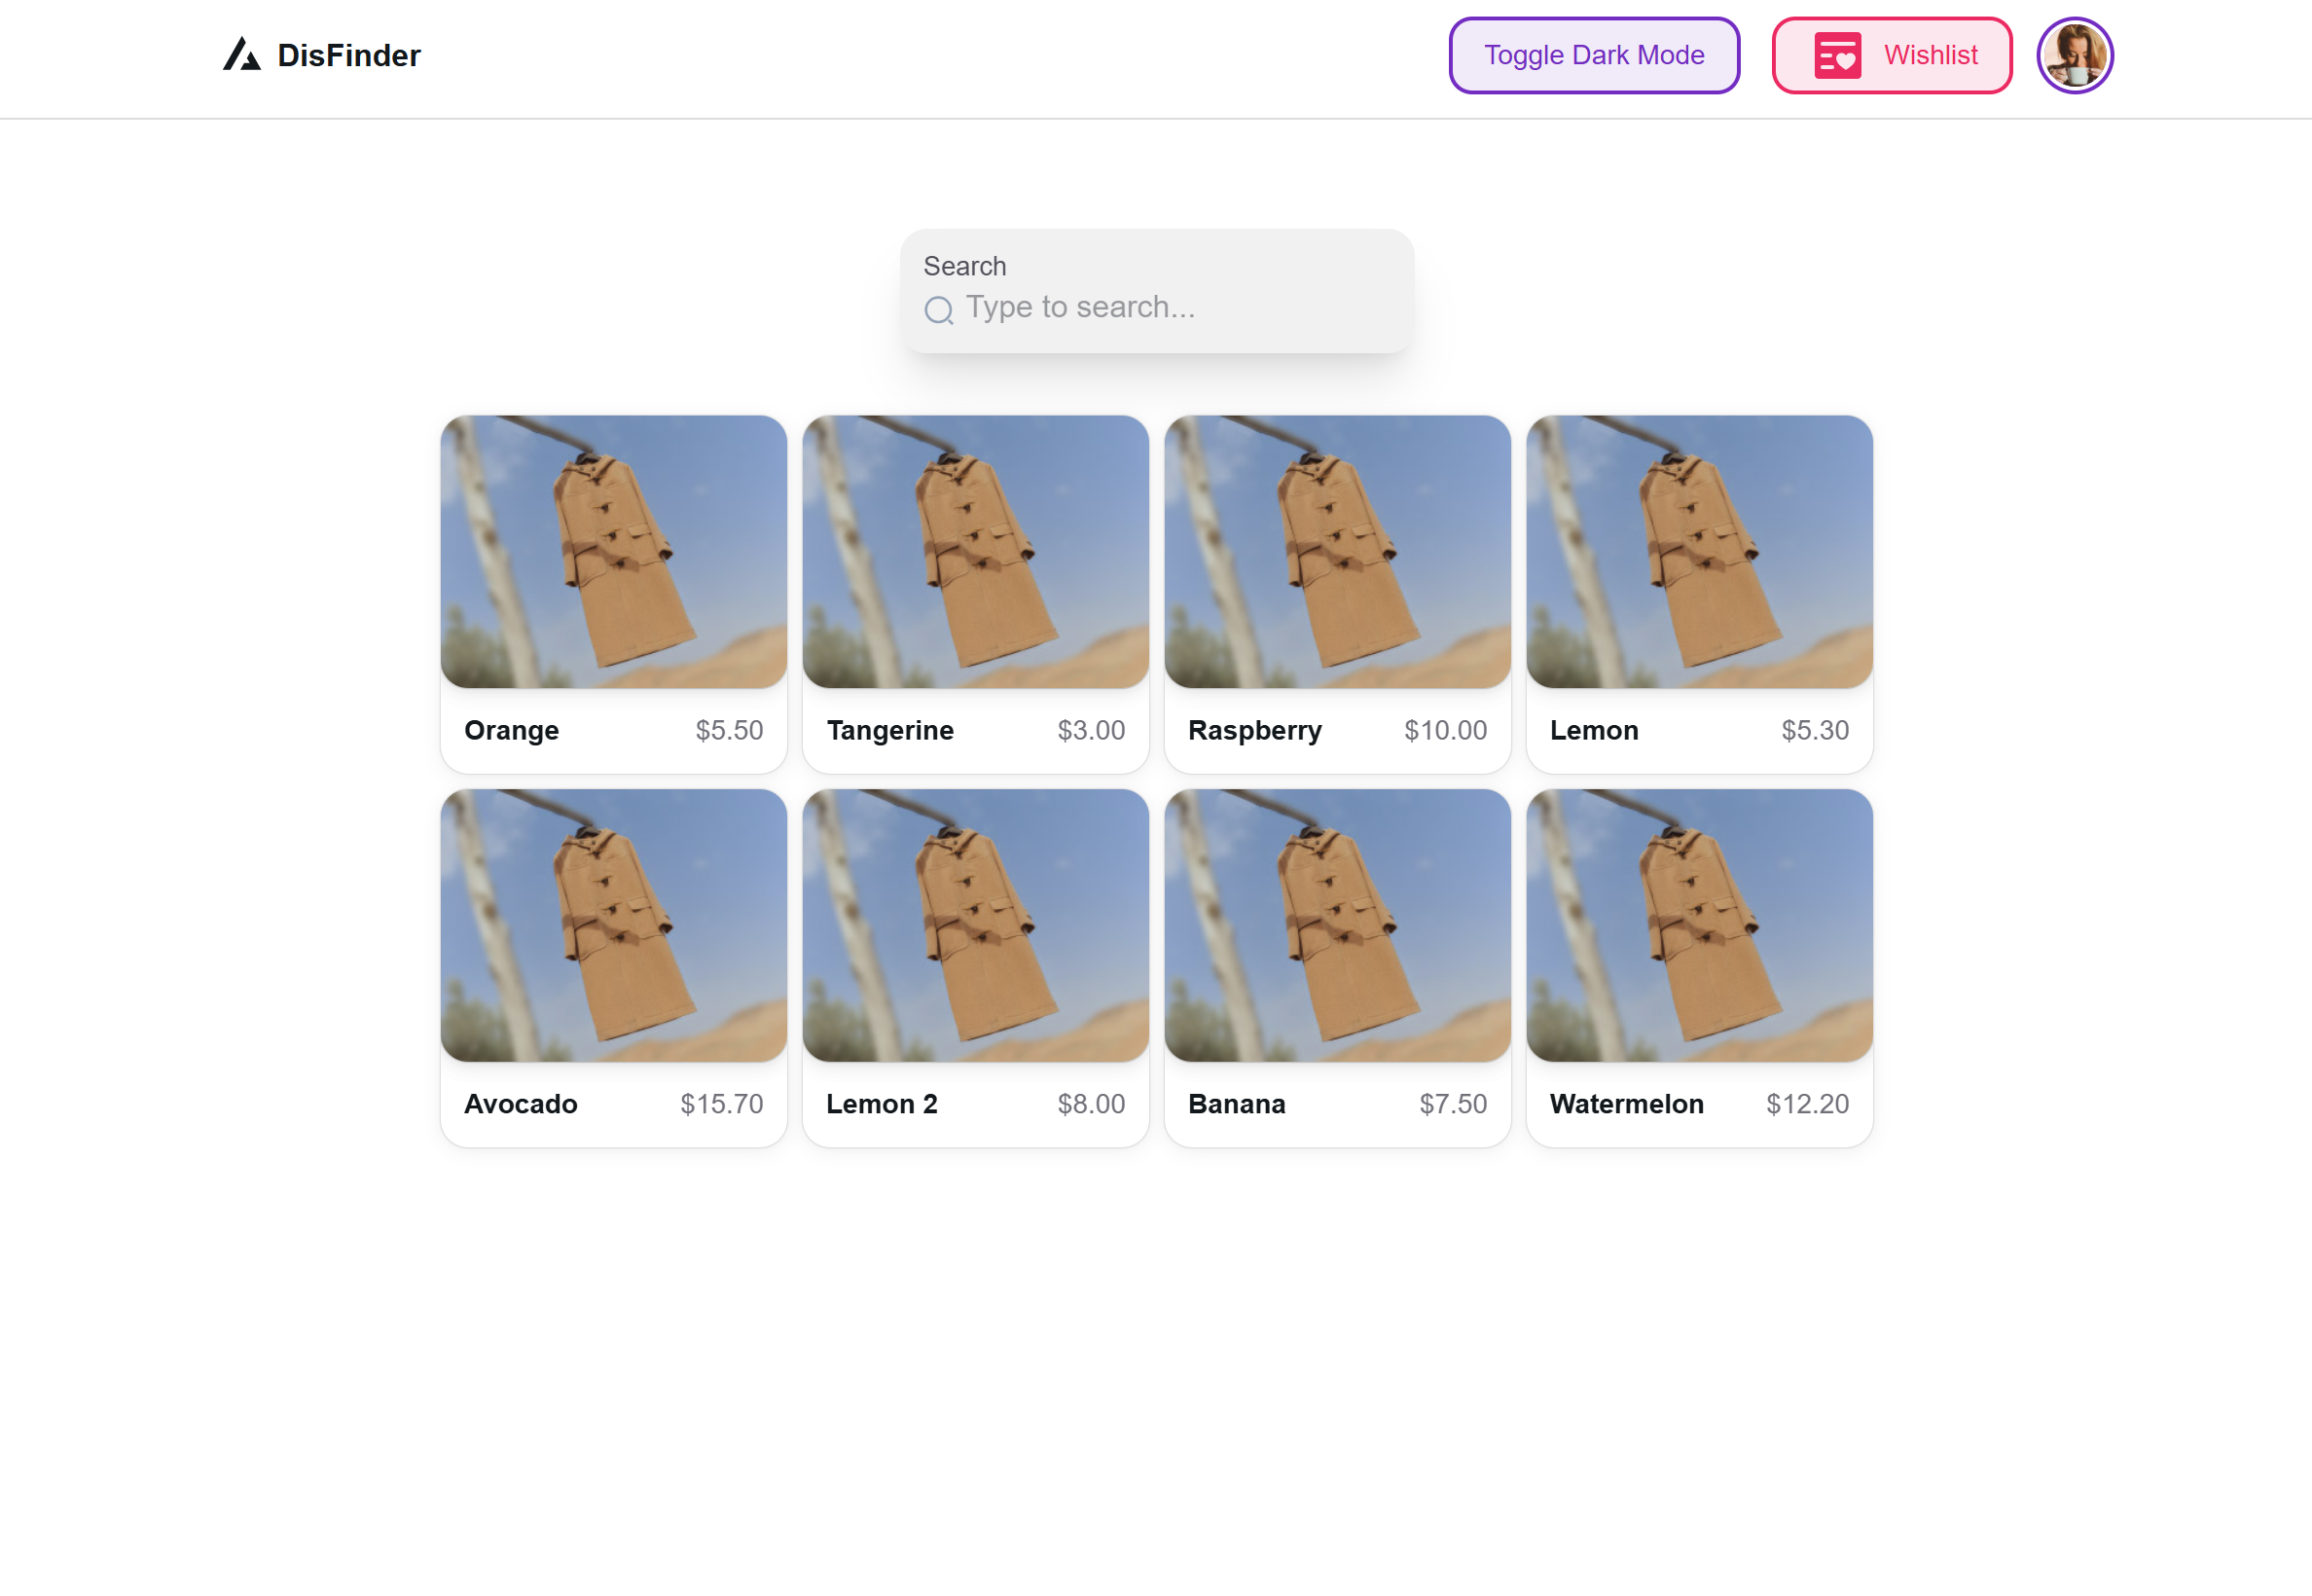
\includegraphics[width=0.5\textwidth]{assets/design/searchpage.png}
\caption{商品搜索界面示例}
\end{figure}

\subsubsection{商品详情界面}

\begin{figure}[H]
\centering
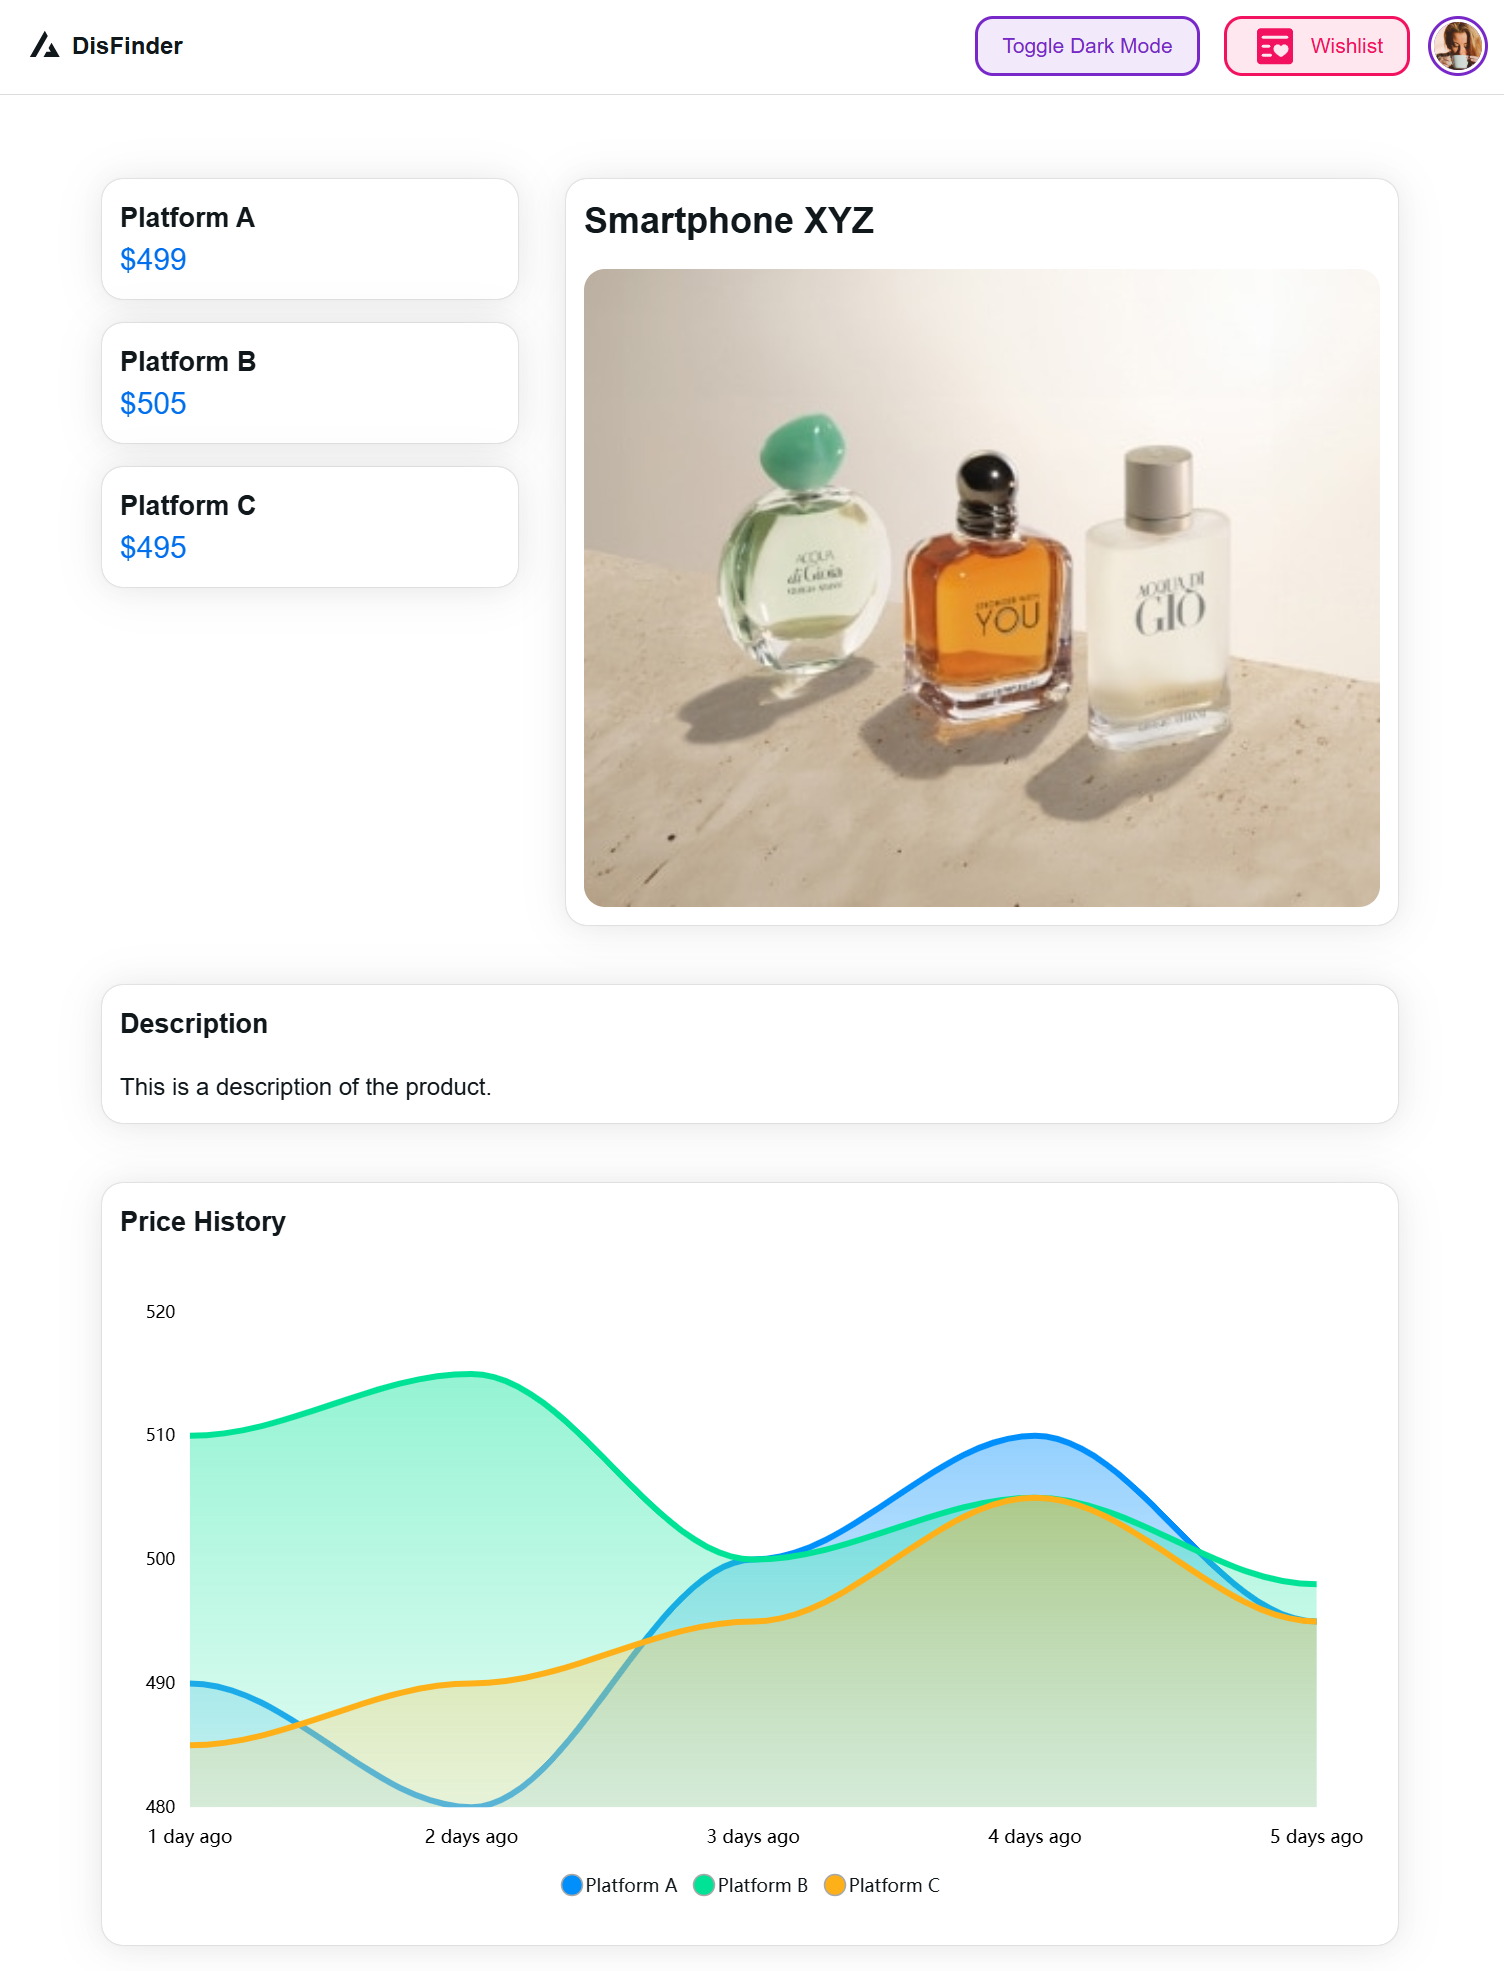
\includegraphics[width=0.5\textwidth]{assets/design/productpage.png}
\caption{商品详情界面示例}
\end{figure}

\subsubsection{心愿单界面}

\begin{figure}[H]
\centering
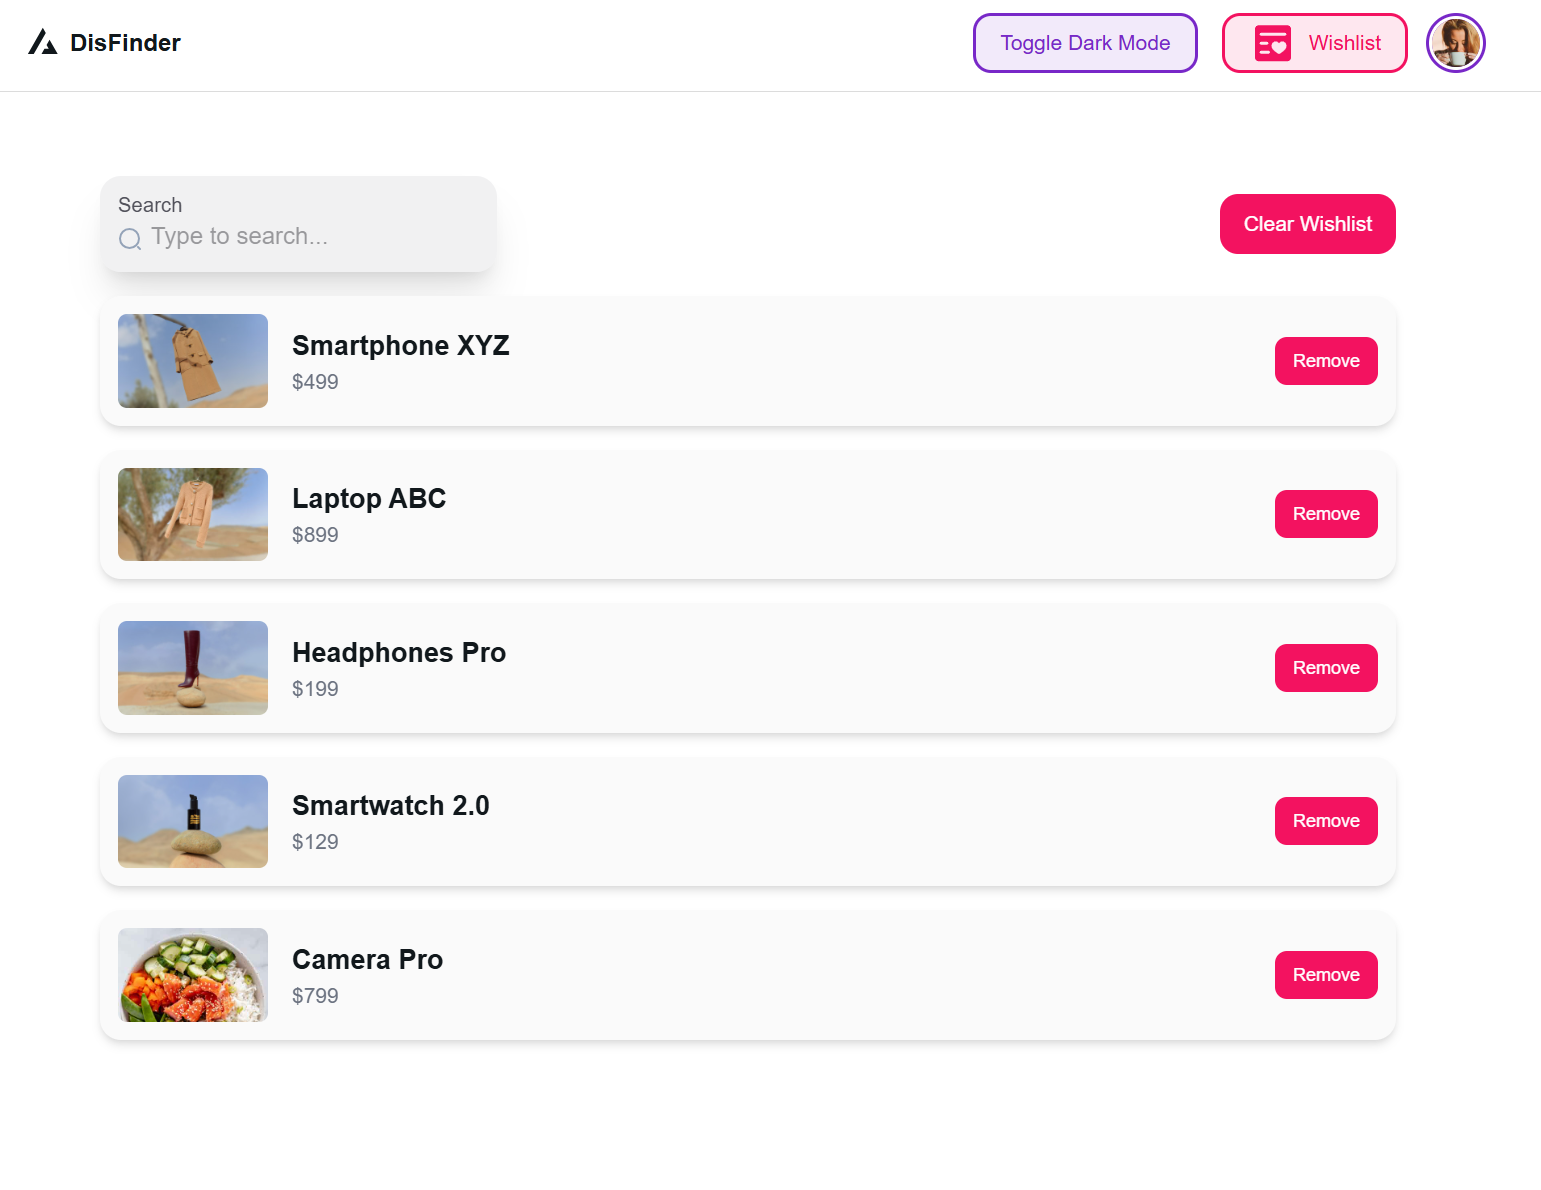
\includegraphics[width=0.5\textwidth]{assets/design/wishlistpage.png}
\caption{心愿单界面示例}
\end{figure}

\subsubsection{夜间模式}

\begin{figure}[H]
\centering
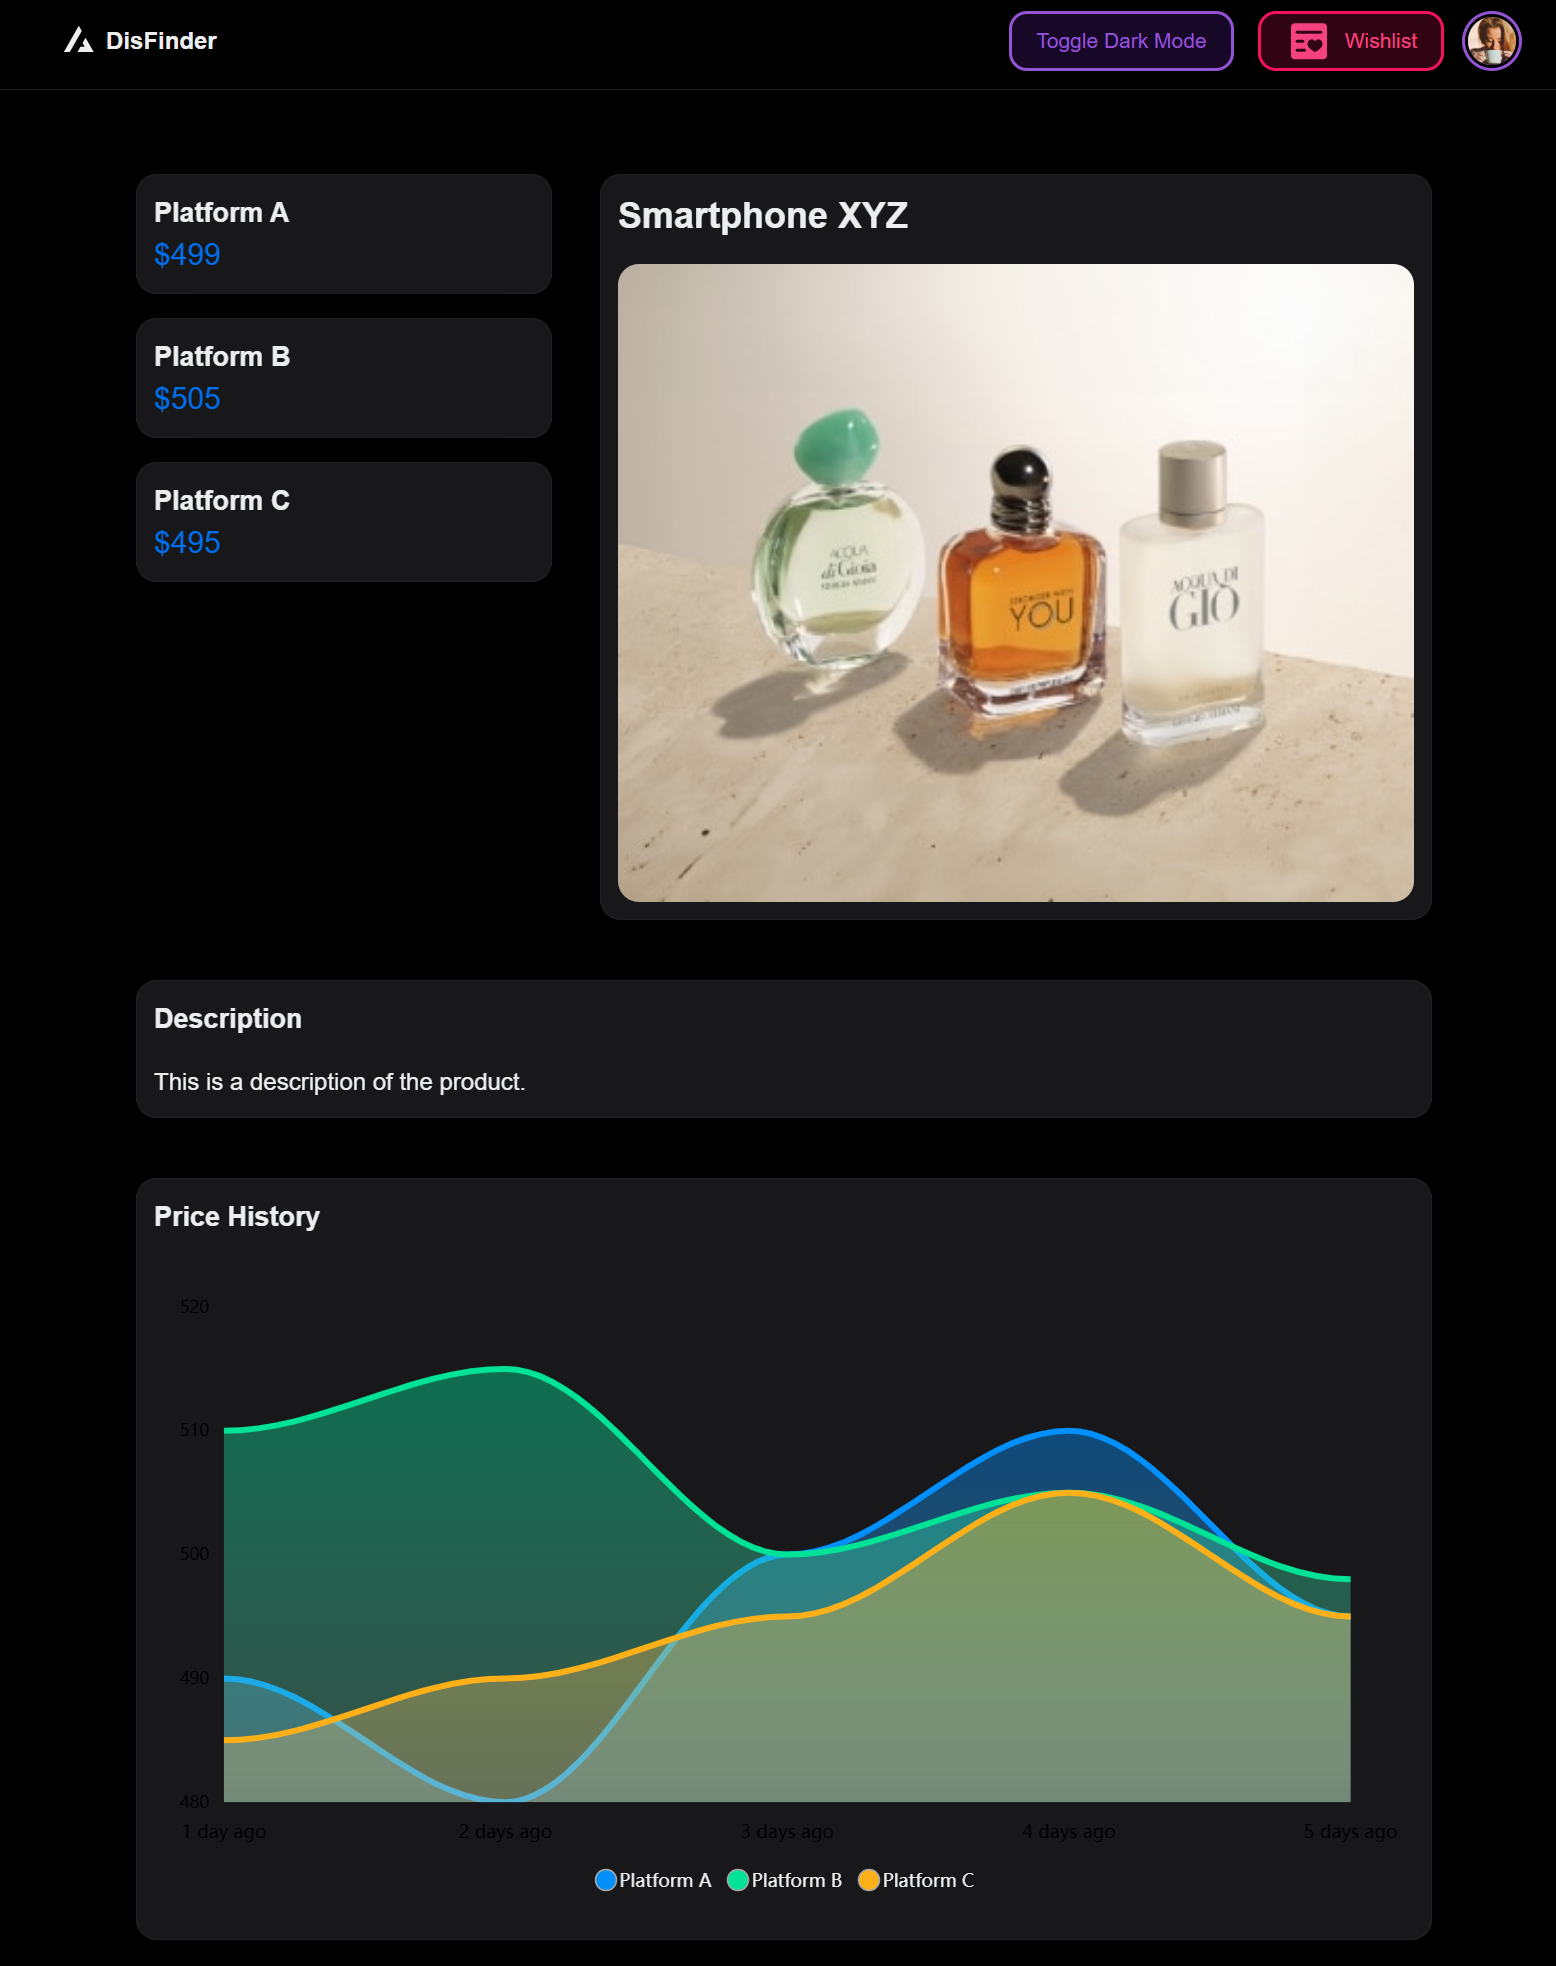
\includegraphics[width=0.5\textwidth]{assets/design/darkmode.png}
\caption{夜间模式示例}
\end{figure}

\chapter{开发计划}

\begin{itemize}
  \item 冬 3 周:完成数据采集模块
  \item 冬 4 周 - 冬 5 周:完成后端,包括 API 响应模块、数据库模块、定时任务模块
  \item 冬 6 周 - 冬 7 周:完成前端,包括页面设计、前端逻辑,并与后端对接
  \item 冬 8 周:测试、部署、优化、完善文档
\end{itemize}
